% Options for packages loaded elsewhere
\PassOptionsToPackage{unicode}{hyperref}
\PassOptionsToPackage{hyphens}{url}
%
\documentclass[
]{article}
\usepackage{lmodern}
\usepackage{amssymb,amsmath}
\usepackage{ifxetex,ifluatex}
\ifnum 0\ifxetex 1\fi\ifluatex 1\fi=0 % if pdftex
  \usepackage[T1]{fontenc}
  \usepackage[utf8]{inputenc}
  \usepackage{textcomp} % provide euro and other symbols
\else % if luatex or xetex
  \usepackage{unicode-math}
  \defaultfontfeatures{Scale=MatchLowercase}
  \defaultfontfeatures[\rmfamily]{Ligatures=TeX,Scale=1}
\fi
% Use upquote if available, for straight quotes in verbatim environments
\IfFileExists{upquote.sty}{\usepackage{upquote}}{}
\IfFileExists{microtype.sty}{% use microtype if available
  \usepackage[]{microtype}
  \UseMicrotypeSet[protrusion]{basicmath} % disable protrusion for tt fonts
}{}
\makeatletter
\@ifundefined{KOMAClassName}{% if non-KOMA class
  \IfFileExists{parskip.sty}{%
    \usepackage{parskip}
  }{% else
    \setlength{\parindent}{0pt}
    \setlength{\parskip}{6pt plus 2pt minus 1pt}}
}{% if KOMA class
  \KOMAoptions{parskip=half}}
\makeatother
\usepackage{xcolor}
\IfFileExists{xurl.sty}{\usepackage{xurl}}{} % add URL line breaks if available
\IfFileExists{bookmark.sty}{\usepackage{bookmark}}{\usepackage{hyperref}}
\hypersetup{
  pdftitle={Cost-Effectiveness and Decision Modeling in R},
  pdfauthor={The DARTH workgroup},
  hidelinks,
  pdfcreator={LaTeX via pandoc}}
\urlstyle{same} % disable monospaced font for URLs
\usepackage[margin=1in]{geometry}
\usepackage{color}
\usepackage{fancyvrb}
\newcommand{\VerbBar}{|}
\newcommand{\VERB}{\Verb[commandchars=\\\{\}]}
\DefineVerbatimEnvironment{Highlighting}{Verbatim}{commandchars=\\\{\}}
% Add ',fontsize=\small' for more characters per line
\usepackage{framed}
\definecolor{shadecolor}{RGB}{248,248,248}
\newenvironment{Shaded}{\begin{snugshade}}{\end{snugshade}}
\newcommand{\AlertTok}[1]{\textcolor[rgb]{0.94,0.16,0.16}{#1}}
\newcommand{\AnnotationTok}[1]{\textcolor[rgb]{0.56,0.35,0.01}{\textbf{\textit{#1}}}}
\newcommand{\AttributeTok}[1]{\textcolor[rgb]{0.77,0.63,0.00}{#1}}
\newcommand{\BaseNTok}[1]{\textcolor[rgb]{0.00,0.00,0.81}{#1}}
\newcommand{\BuiltInTok}[1]{#1}
\newcommand{\CharTok}[1]{\textcolor[rgb]{0.31,0.60,0.02}{#1}}
\newcommand{\CommentTok}[1]{\textcolor[rgb]{0.56,0.35,0.01}{\textit{#1}}}
\newcommand{\CommentVarTok}[1]{\textcolor[rgb]{0.56,0.35,0.01}{\textbf{\textit{#1}}}}
\newcommand{\ConstantTok}[1]{\textcolor[rgb]{0.00,0.00,0.00}{#1}}
\newcommand{\ControlFlowTok}[1]{\textcolor[rgb]{0.13,0.29,0.53}{\textbf{#1}}}
\newcommand{\DataTypeTok}[1]{\textcolor[rgb]{0.13,0.29,0.53}{#1}}
\newcommand{\DecValTok}[1]{\textcolor[rgb]{0.00,0.00,0.81}{#1}}
\newcommand{\DocumentationTok}[1]{\textcolor[rgb]{0.56,0.35,0.01}{\textbf{\textit{#1}}}}
\newcommand{\ErrorTok}[1]{\textcolor[rgb]{0.64,0.00,0.00}{\textbf{#1}}}
\newcommand{\ExtensionTok}[1]{#1}
\newcommand{\FloatTok}[1]{\textcolor[rgb]{0.00,0.00,0.81}{#1}}
\newcommand{\FunctionTok}[1]{\textcolor[rgb]{0.00,0.00,0.00}{#1}}
\newcommand{\ImportTok}[1]{#1}
\newcommand{\InformationTok}[1]{\textcolor[rgb]{0.56,0.35,0.01}{\textbf{\textit{#1}}}}
\newcommand{\KeywordTok}[1]{\textcolor[rgb]{0.13,0.29,0.53}{\textbf{#1}}}
\newcommand{\NormalTok}[1]{#1}
\newcommand{\OperatorTok}[1]{\textcolor[rgb]{0.81,0.36,0.00}{\textbf{#1}}}
\newcommand{\OtherTok}[1]{\textcolor[rgb]{0.56,0.35,0.01}{#1}}
\newcommand{\PreprocessorTok}[1]{\textcolor[rgb]{0.56,0.35,0.01}{\textit{#1}}}
\newcommand{\RegionMarkerTok}[1]{#1}
\newcommand{\SpecialCharTok}[1]{\textcolor[rgb]{0.00,0.00,0.00}{#1}}
\newcommand{\SpecialStringTok}[1]{\textcolor[rgb]{0.31,0.60,0.02}{#1}}
\newcommand{\StringTok}[1]{\textcolor[rgb]{0.31,0.60,0.02}{#1}}
\newcommand{\VariableTok}[1]{\textcolor[rgb]{0.00,0.00,0.00}{#1}}
\newcommand{\VerbatimStringTok}[1]{\textcolor[rgb]{0.31,0.60,0.02}{#1}}
\newcommand{\WarningTok}[1]{\textcolor[rgb]{0.56,0.35,0.01}{\textbf{\textit{#1}}}}
\usepackage{longtable,booktabs}
% Correct order of tables after \paragraph or \subparagraph
\usepackage{etoolbox}
\makeatletter
\patchcmd\longtable{\par}{\if@noskipsec\mbox{}\fi\par}{}{}
\makeatother
% Allow footnotes in longtable head/foot
\IfFileExists{footnotehyper.sty}{\usepackage{footnotehyper}}{\usepackage{footnote}}
\makesavenoteenv{longtable}
\usepackage{graphicx,grffile}
\makeatletter
\def\maxwidth{\ifdim\Gin@nat@width>\linewidth\linewidth\else\Gin@nat@width\fi}
\def\maxheight{\ifdim\Gin@nat@height>\textheight\textheight\else\Gin@nat@height\fi}
\makeatother
% Scale images if necessary, so that they will not overflow the page
% margins by default, and it is still possible to overwrite the defaults
% using explicit options in \includegraphics[width, height, ...]{}
\setkeys{Gin}{width=\maxwidth,height=\maxheight,keepaspectratio}
% Set default figure placement to htbp
\makeatletter
\def\fps@figure{htbp}
\makeatother
\setlength{\emergencystretch}{3em} % prevent overfull lines
\providecommand{\tightlist}{%
  \setlength{\itemsep}{0pt}\setlength{\parskip}{0pt}}
\setcounter{secnumdepth}{-\maxdimen} % remove section numbering

\title{Cost-Effectiveness and Decision Modeling in R}
\usepackage{etoolbox}
\makeatletter
\providecommand{\subtitle}[1]{% add subtitle to \maketitle
  \apptocmd{\@title}{\par {\large #1 \par}}{}{}
}
\makeatother
\subtitle{Exercises -- Survival analysis in Decision modeling}
\author{The DARTH workgroup}
\date{}

\begin{document}
\maketitle

Developed by the Decision Analysis in R for Technologies in Health
(DARTH) workgroup:

Fernando Alarid-Escudero, PhD (1)

Eva A. Enns, MS, PhD (2)

M.G. Myriam Hunink, MD, PhD (3,4)

Hawre J. Jalal, MD, PhD (5)

Eline M. Krijkamp, MSc (3)

Petros Pechlivanoglou, PhD (6)

Alan Yang, MSc (7)

In collaboration of:

\begin{enumerate}
\def\labelenumi{\arabic{enumi}.}
\tightlist
\item
  Drug Policy Program, Center for Research and Teaching in Economics
  (CIDE) - CONACyT, Aguascalientes, Mexico
\item
  University of Minnesota School of Public Health, Minneapolis, MN, USA
\item
  Erasmus MC, Rotterdam, The Netherlands
\item
  Harvard T.H. Chan School of Public Health, Boston, USA
\item
  University of Pittsburgh Graduate School of Public Health, Pittsburgh,
  PA, USA
\item
  The Hospital for Sick Children, Toronto and University of Toronto,
  Toronto ON, Canada
\item
  The Hospital for Sick Children, Toronto ON, Canada
\end{enumerate}

Please cite our publications when using this code:

\begin{itemize}
\item
  Jalal H, Pechlivanoglou P, Krijkamp E, Alarid-Escudero F, Enns E,
  Hunink MG. An Overview of R in Health Decision Sciences. Med Decis
  Making. 2017; 37(3): 735-746.
  \url{https://journals.sagepub.com/doi/abs/10.1177/0272989X16686559}
\item
  Krijkamp EM, Alarid-Escudero F, Enns EA, Jalal HJ, Hunink MGM,
  Pechlivanoglou P. Microsimulation modeling for health decision
  sciences using R: A tutorial. Med Decis Making. 2018;38(3):400--22.
  \url{https://journals.sagepub.com/doi/abs/10.1177/0272989X18754513}
\item
  Krijkamp EM, Alarid-Escudero F, Enns E, Pechlivanoglou P, Hunink MM,
  Jalal H. A Multidimensional Array Representation of State-Transition
  Model Dynamics. BioRxiv 670612
  2019.https://www.biorxiv.org/content/10.1101/670612v1
\end{itemize}

Copyright 2017, THE HOSPITAL FOR SICK CHILDREN AND THE COLLABORATING
INSTITUTIONS. All rights reserved in Canada, the United States and
worldwide. Copyright, trademarks, trade names and any and all associated
intellectual property are exclusively owned by THE HOSPITAL FOR Sick
CHILDREN and the collaborating institutions. These materials may be
used, reproduced, modified, distributed and adapted with proper
attribution.

\hypertarget{exercise-a-microsimulation-model-the-sick-sicker-model}{%
\section{Exercise: A Microsimulation model -- The Sick-Sicker
model}\label{exercise-a-microsimulation-model-the-sick-sicker-model}}

In this exercise, we will model a hypothetical disease that affects
individuals with an average age of 25 years and results in increased
mortality, increased healthcare costs, and reduced quality of life. The
disease has two levels; affected individuals initially become sick but
can subsequently progress and become sicker. Two alternative strategies
exist for this hypothetical disease: a no-treatment and a treatment
strategy. Under the treatment strategy, individuals in the sick and
sicker states are treated until they recover (only if sick; individuals
in the sicker state cannot recover) or die. The cost of the treatment is
additive to the baseline healthcare costs of being sick or sicker. The
treatment improves quality of life for those individuals who are sick
but has no impact on the quality of life of those who are sicker.
Unfortunately, it is not possible to reliably differentiate between
people in the sick and sicker states, so treatment cannot be targeted to
only those in the sick state. You are asked to evaluate the
cost-effectiveness of the treatment.

To model this disease, we will rely on a microsimulation model, called
the Sick-Sicker model, first described by Enns et al.~The Sick-Sicker
model consists of four health states: Healthy (H), two disease states,
Sick (S1) and Sicker (S2), and Dead (D) (Figure 1). All individuals
start in the Healthy state. Over time, healthy individuals may develop
the disease and can progress to S1. Individuals in S1 can recover
(return to state H), progress further to S2 or die. Individuals in S2
cannot recover (i.e.~cannot transition to either S1 or H). Individuals
in H have a baseline probability of death; individuals in S1 and S2
experience increased mortality compared to those in the H state, given
in terms of hazard ratios. These ratios are used to calculate the
probabilities of dying when in S1 and S2.

You were given access to individual-level data of patients with the
hypothetical disease. From the data you are asked to inform the
transition probabilities for the transitions from S1 to H, from S1 to S2
and from S1 to D directly from the data through the use of parametric
survival functions. A snapshot of the data is presented below:

\begin{Shaded}
\begin{Highlighting}[]
\NormalTok{data_long <-}\StringTok{ }\KeywordTok{read.csv}\NormalTok{(here}\OperatorTok{::}\KeywordTok{here}\NormalTok{(}\StringTok{"data"}\NormalTok{, }\StringTok{"data_long_Sicker.csv"}\NormalTok{), }\DataTypeTok{row.names =} \DecValTok{1}\NormalTok{)}
\KeywordTok{head}\NormalTok{(data_long)}
\end{Highlighting}
\end{Shaded}

\begin{verbatim}
##   id from to trans Tstart      Tstop       time status
## 1  1   S1  H     1      0 1.33364908 1.33364908      1
## 2  1   S1 S2     2      0 1.33364908 1.33364908      0
## 3  1   S1  D     3      0 1.33364908 1.33364908      0
## 4  2   S1  H     1      0 0.05171561 0.05171561      1
## 5  2   S1 S2     2      0 0.05171561 0.05171561      0
## 6  2   S1  D     3      0 0.05171561 0.05171561      0
\end{verbatim}

\hypertarget{tasks}{%
\subsection{Tasks}\label{tasks}}

\textbf{Part 1}

\begin{enumerate}
\def\labelenumi{\arabic{enumi}.}
\item
  Use the \texttt{R} script ``Surv\_Sick\_Sicker\_template.R'' as a
  starting point to code the survival analysis solution to the
  Sick-Sicker model.
\item
  Load the individual level data in long form from the
  \texttt{data\_long\_Sicker.csv} file.
\item
  Subset the data by transition so that you can fit separate models for
  each transition.
\item
  Draw Kaplan Meier plots for each transition.
\item
  Estimate parametric distributions to the patient level survival data
  for all data-informed transitions.
\item
  Select the one with the most plausible fit (both clinically and
  statistically).
\end{enumerate}

\textbf{OPTIONAL}

\begin{enumerate}
\def\labelenumi{\arabic{enumi}.}
\item
  Incorporate the transition probabilities extracted from the survival
  analysis model to the Sick Sicker time microsimulation. HINT:
  Depending on the distribution you choose you will need to track more
  time-in-state variables.
\item
  Run the microsimulation model and draw output from it.
\end{enumerate}

\textbf{Table 1: Input parameters for the time dependent Sick-Sicker
Microsimulation }

\begin{longtable}[]{@{}llc@{}}
\toprule
\begin{minipage}[b]{0.51\columnwidth}\raggedright
\textbf{Parameter}\strut
\end{minipage} & \begin{minipage}[b]{0.19\columnwidth}\raggedright
\textbf{R name}\strut
\end{minipage} & \begin{minipage}[b]{0.21\columnwidth}\centering
\textbf{Value}\strut
\end{minipage}\tabularnewline
\midrule
\endhead
\begin{minipage}[t]{0.51\columnwidth}\raggedright
Time horizon\strut
\end{minipage} & \begin{minipage}[t]{0.19\columnwidth}\raggedright
\texttt{n\_t}\strut
\end{minipage} & \begin{minipage}[t]{0.21\columnwidth}\centering
30 years\strut
\end{minipage}\tabularnewline
\begin{minipage}[t]{0.51\columnwidth}\raggedright
Cycle length\strut
\end{minipage} & \begin{minipage}[t]{0.19\columnwidth}\raggedright
\strut
\end{minipage} & \begin{minipage}[t]{0.21\columnwidth}\centering
1 year\strut
\end{minipage}\tabularnewline
\begin{minipage}[t]{0.51\columnwidth}\raggedright
Names of simulated individuals\strut
\end{minipage} & \begin{minipage}[t]{0.19\columnwidth}\raggedright
\texttt{n\_i}\strut
\end{minipage} & \begin{minipage}[t]{0.21\columnwidth}\centering
1000\strut
\end{minipage}\tabularnewline
\begin{minipage}[t]{0.51\columnwidth}\raggedright
Names of health states\strut
\end{minipage} & \begin{minipage}[t]{0.19\columnwidth}\raggedright
\texttt{v\_n}\strut
\end{minipage} & \begin{minipage}[t]{0.21\columnwidth}\centering
H, S1, S2, D\strut
\end{minipage}\tabularnewline
\begin{minipage}[t]{0.51\columnwidth}\raggedright
Annual discount rate (costs/QALYs)\strut
\end{minipage} & \begin{minipage}[t]{0.19\columnwidth}\raggedright
\texttt{d\_r}\strut
\end{minipage} & \begin{minipage}[t]{0.21\columnwidth}\centering
3\%\strut
\end{minipage}\tabularnewline
\begin{minipage}[t]{0.51\columnwidth}\raggedright
Population characteristics\strut
\end{minipage} & \begin{minipage}[t]{0.19\columnwidth}\raggedright
\strut
\end{minipage} & \begin{minipage}[t]{0.21\columnwidth}\centering
\strut
\end{minipage}\tabularnewline
\begin{minipage}[t]{0.51\columnwidth}\raggedright
- Agedistribution\strut
\end{minipage} & \begin{minipage}[t]{0.19\columnwidth}\raggedright
--\strut
\end{minipage} & \begin{minipage}[t]{0.21\columnwidth}\centering
Range:25-55 distributed as in
\texttt{MyPopulation-AgeDistribution.csv}\strut
\end{minipage}\tabularnewline
\begin{minipage}[t]{0.51\columnwidth}\raggedright
Annual transition probabilities\strut
\end{minipage} & \begin{minipage}[t]{0.19\columnwidth}\raggedright
\strut
\end{minipage} & \begin{minipage}[t]{0.21\columnwidth}\centering
\strut
\end{minipage}\tabularnewline
\begin{minipage}[t]{0.51\columnwidth}\raggedright
- Disease onset (H to S1)\strut
\end{minipage} & \begin{minipage}[t]{0.19\columnwidth}\raggedright
\texttt{p\_HS1}\strut
\end{minipage} & \begin{minipage}[t]{0.21\columnwidth}\centering
0.15\strut
\end{minipage}\tabularnewline
\begin{minipage}[t]{0.51\columnwidth}\raggedright
Annual mortality\strut
\end{minipage} & \begin{minipage}[t]{0.19\columnwidth}\raggedright
\strut
\end{minipage} & \begin{minipage}[t]{0.21\columnwidth}\centering
\strut
\end{minipage}\tabularnewline
\begin{minipage}[t]{0.51\columnwidth}\raggedright
- All-cause mortality (H to D)\strut
\end{minipage} & \begin{minipage}[t]{0.19\columnwidth}\raggedright
\texttt{p\_HD}\strut
\end{minipage} & \begin{minipage}[t]{0.21\columnwidth}\centering
Human Mortality Database: age dependent from 2015\strut
\end{minipage}\tabularnewline
\begin{minipage}[t]{0.51\columnwidth}\raggedright
Annual costs\strut
\end{minipage} & \begin{minipage}[t]{0.19\columnwidth}\raggedright
\strut
\end{minipage} & \begin{minipage}[t]{0.21\columnwidth}\centering
\strut
\end{minipage}\tabularnewline
\begin{minipage}[t]{0.51\columnwidth}\raggedright
- Healthy individuals\strut
\end{minipage} & \begin{minipage}[t]{0.19\columnwidth}\raggedright
\texttt{c\_H}\strut
\end{minipage} & \begin{minipage}[t]{0.21\columnwidth}\centering
\$2,000\strut
\end{minipage}\tabularnewline
\begin{minipage}[t]{0.51\columnwidth}\raggedright
- Sick individuals in S1\strut
\end{minipage} & \begin{minipage}[t]{0.19\columnwidth}\raggedright
\texttt{c\_S1}\strut
\end{minipage} & \begin{minipage}[t]{0.21\columnwidth}\centering
\$4,000\strut
\end{minipage}\tabularnewline
\begin{minipage}[t]{0.51\columnwidth}\raggedright
- Sick individuals in S2\strut
\end{minipage} & \begin{minipage}[t]{0.19\columnwidth}\raggedright
\texttt{c\_S2}\strut
\end{minipage} & \begin{minipage}[t]{0.21\columnwidth}\centering
\$15,000\strut
\end{minipage}\tabularnewline
\begin{minipage}[t]{0.51\columnwidth}\raggedright
- Dead individuals\strut
\end{minipage} & \begin{minipage}[t]{0.19\columnwidth}\raggedright
\texttt{c\_D}\strut
\end{minipage} & \begin{minipage}[t]{0.21\columnwidth}\centering
\$0\strut
\end{minipage}\tabularnewline
\begin{minipage}[t]{0.51\columnwidth}\raggedright
- Additional costs of sick individuals treated in S1 or S2\strut
\end{minipage} & \begin{minipage}[t]{0.19\columnwidth}\raggedright
\texttt{c\_trt}\strut
\end{minipage} & \begin{minipage}[t]{0.21\columnwidth}\centering
\$12,000\strut
\end{minipage}\tabularnewline
\begin{minipage}[t]{0.51\columnwidth}\raggedright
Utility weights\strut
\end{minipage} & \begin{minipage}[t]{0.19\columnwidth}\raggedright
\strut
\end{minipage} & \begin{minipage}[t]{0.21\columnwidth}\centering
\strut
\end{minipage}\tabularnewline
\begin{minipage}[t]{0.51\columnwidth}\raggedright
- Healthy individuals\strut
\end{minipage} & \begin{minipage}[t]{0.19\columnwidth}\raggedright
\texttt{u\_H}\strut
\end{minipage} & \begin{minipage}[t]{0.21\columnwidth}\centering
1.00\strut
\end{minipage}\tabularnewline
\begin{minipage}[t]{0.51\columnwidth}\raggedright
- Sick individuals in S1\strut
\end{minipage} & \begin{minipage}[t]{0.19\columnwidth}\raggedright
\texttt{u\_S1}\strut
\end{minipage} & \begin{minipage}[t]{0.21\columnwidth}\centering
0.75\strut
\end{minipage}\tabularnewline
\begin{minipage}[t]{0.51\columnwidth}\raggedright
- Sick individuals in S2\strut
\end{minipage} & \begin{minipage}[t]{0.19\columnwidth}\raggedright
\texttt{u\_S2}\strut
\end{minipage} & \begin{minipage}[t]{0.21\columnwidth}\centering
0.50\strut
\end{minipage}\tabularnewline
\begin{minipage}[t]{0.51\columnwidth}\raggedright
- Dead individuals\strut
\end{minipage} & \begin{minipage}[t]{0.19\columnwidth}\raggedright
\texttt{u\_D}\strut
\end{minipage} & \begin{minipage}[t]{0.21\columnwidth}\centering
0.00\strut
\end{minipage}\tabularnewline
\begin{minipage}[t]{0.51\columnwidth}\raggedright
Intervention effect\strut
\end{minipage} & \begin{minipage}[t]{0.19\columnwidth}\raggedright
\strut
\end{minipage} & \begin{minipage}[t]{0.21\columnwidth}\centering
\strut
\end{minipage}\tabularnewline
\begin{minipage}[t]{0.51\columnwidth}\raggedright
- Utility for treated individuals in S1\strut
\end{minipage} & \begin{minipage}[t]{0.19\columnwidth}\raggedright
\texttt{u\_trt}\strut
\end{minipage} & \begin{minipage}[t]{0.21\columnwidth}\centering
0.95\strut
\end{minipage}\tabularnewline
\begin{minipage}[t]{0.51\columnwidth}\raggedright
Time varying extension of Sick-Sicker model\strut
\end{minipage} & \begin{minipage}[t]{0.19\columnwidth}\raggedright
\strut
\end{minipage} & \begin{minipage}[t]{0.21\columnwidth}\centering
\strut
\end{minipage}\tabularnewline
\begin{minipage}[t]{0.51\columnwidth}\raggedright
- Treatment effect modifier at baseline\strut
\end{minipage} & \begin{minipage}[t]{0.19\columnwidth}\raggedright
\texttt{v\_x}\strut
\end{minipage} & \begin{minipage}[t]{0.21\columnwidth}\centering
Uniform(0.95, 1.05)\strut
\end{minipage}\tabularnewline
\bottomrule
\end{longtable}

\begin{figure}

{\centering 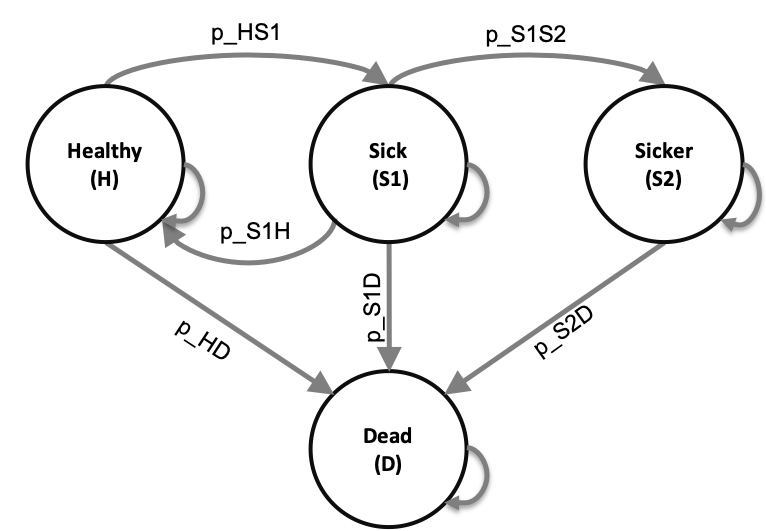
\includegraphics[width=1\linewidth]{C:/Users/Alan Yang/Desktop/GitHub local/Course-Modularization/static/Course_Modularization/Survival analysis/Survival Sick-Sicker/figures/sick_sicker_diagram} 

}

\caption{Schematic representation of the Sick-Sicker model}\label{fig:unnamed-chunk-2}
\end{figure}

\end{document}
